\documentclass[11pt, letterpaper]{amsart}
\usepackage[utf8]{inputenc}

%%%% ADDING CODE PACKAGE

\usepackage{listings}
\usepackage{color}

\definecolor{dkgreen}{rgb}{0,0.6,0}
\definecolor{gray}{rgb}{0.5,0.5,0.5}
\definecolor{mauve}{rgb}{0.58,0,0.82}

\lstset{frame=tb,
  language=Python,
  aboveskip=3mm,
  belowskip=3mm,
  showstringspaces=false,
  columns=flexible,
  basicstyle={\small\ttfamily},
  numbers=none,
  numberstyle=\tiny\color{gray},
  keywordstyle=\color{blue},
  commentstyle=\color{dkgreen},
  stringstyle=\color{mauve},
  breaklines=true,
  breakatwhitespace=true,
  tabsize=3
}

\usepackage{graphicx}
\usepackage{caption}
\usepackage{subcaption}

\usepackage{amsmath}
\usepackage{amssymb}
\usepackage{float}
\usepackage[]{algorithm2e}
\restylefloat{table}
\usepackage{amsthm} % For theorems.
\usepackage[hidelinks]{hyperref} %For hyperlinks, [hidelinks] is to take away link boarders.

\usepackage{csquotes} % Used for displaying the quote using \begin{displayquote}

\usepackage{mathtools} % in order tp use \coloneqq

\begin{document}

\begin{titlepage}
\begin{center}

\includegraphics[scale=0.2]{LundUniversity_C2line_BLACK.png}

\vspace{1cm}

\Large{Feedforward neural networks with ReLU activation functions are linear splines}

\vspace{0.5cm}

\large{Magnus Hansson $\&$ Christoffer Olsson}

\small{hansson.carl.magnus@gmail.com}
\small{olschr2@gmail.com}

\vspace{1cm}

supervised by\par 
Najmeh Abiri $\&$ Claus Führer


\vspace{1cm}

\large{August 2017}

\vspace{1cm}

\small{Department of Numerical Analysis}
\\
\small{Lund University}

\vspace{1cm}

\end{center}
\small{\textbf{Abstract.} In this thesis the approximation properties of feedforward artificial neural networks with one hidden layer and ReLU activation functions are examined. It is shown that functions of these kind are linear splines and the number of spline knots depend on the number of nodes in the network. In fact an upper bound can be derived for the number of knots. Furthermore, the positioning of the knots depend on the optimization of the adjustable parameters of the network. A numerical example is given where the network models are compared to linear interpolating splines with equidistant positioned knots.
\vfill


\small{\textbf{Key words:} artificial neural networks, ReLU, splines}
\end{titlepage}

\newpage

\section*{Populärvetenskaplig sammanfattning på svenska}
Artificiella neurala nätverk tillhör en framväxande tvärvetenskaplig gren av matematik, statistik och datavetenskap kallad maskininlärning. Dessa nätverk är från början inspirerade av en biologisk hjärna. Både den artificiella hjärnan och den biologiska hjärnan består utav neuroner som är sammankopplade, ju fler neuroner desto mer komplext och snabbt blir systemet. På samma sätt som en biologisk hjärna lär sig av erfarenhet lär sig ett artificiellt neuralt nätverk av erfarenhet, men i form av observerade datapunkter inlästa i en dator. En artificiell hjärna kan precis som en biologisk lära sig att köra en bil ifall komplexiteten är tillräckligt hög och tillräckligt med erfarenhet, även kallat träning, ges. I dag ser vi dessa nätverk användas dolt inom diverse områden i vår vardag, till exempel datorapplikationer som bildigenkänning.
\\

I denna uppsats undersöks hur ett specifikt nätverk kan förklaras och sammankopplas med befintliga konventionella koncept inom den matematiska grenen numerisk analys. Två ansatser, gällande nätverkets approximationssätt, är anförda i uppsatsen och sedermera bevisade. Satserna förklarar hur det artificiella neurala nätverket bedriver sin generalisering av träningen och lär sig efterlikna underliggande funktioner genom ett styckvist definierat linjärt system, kallat i matematiken, \textit{linjära splines}.

\newpage

\tableofcontents
\newpage

\section*{Author's preface}
As understood it is not too common that two students collaborate in writing their Bachelor's thesis in mathematics. That said, we are grateful to our supervisors Najmeh Abiri and Claus Führer who from the beginning of the project have been encouraging. Since the start we have lived by the philosophy of full transparency and whatever knowledge one acquired everyone in the project needed to fully understand. This has been especially important since the subject of neural networks is an interdisciplinary subject with its roots in mathematics, statistics, numerical analysis and computer science.
\\

Since starting the project in November 2016 we have iteratively understood the subject more and more comprehensively. The field of neural networks is extremely wide. Most commonly they are used as a tool to do regression, classification or predictions within machine learning. One of the major challenges has been to pick a sufficiently small sub-field within the literature to investigate. One of the reasons why this has been a difficult task is because in order to choose something precise one has to understand the field thoroughly.
\\

After understanding the mathematics and the mechanics behind the neural network, a natural way forward was to start programming and experimenting, which was a large part of our learning curve. We discovered how neural networks could be used for approximation, regression and classification within machine learning. When the larger picture was starting to clarify our interest shifted into the questions such as \textit{How are artificial neural networks really connected to mathematics, or more precisely, approximation theory and numerical analysis?} Digging deeper into these questions we understood that by answering a small part of these questions artificial neural networks could easier be explained to mathematicians familiar with numerical analysis.
\\

During Christmas we discovered a paper by Kevin K. Chen, \textit{The upper bound on knots in neural networks} (Chen 2016), we understood how we could connect neural networks to numerical analysis, and in particular spline theory.

\newpage


\section*{Glossary}
\noindent
\textbf{Artificial neural network} $\cdots$ A numerical method inspired by the structure of the biological neural network. In the most general definition it would be a mapping from $\mathbb{R}^n \rightarrow \mathbb{R}^m$. Where $n$ and $m$ are natural numbers.
\\

\noindent
\textbf{Activation function} $\cdots$ In neural networks the modelling of the activation function is inspired by neurology, where information is sent to a biological neuron. The neuron has some kind of activation, which fires a signal to connected neurons if the neuron gets stimulated. An activation function is wrapped around each node or neuron in the artificial neural network. The activation function gives the neural network its characteristics, i.e, e.g, if the neural network yields a regression or a classification.
\\

\noindent
\textbf{Backpropagation} $\cdots$ A method in which the gradient of the error function of a neural network is calculated. Backpropagation is used in the optimization process of the error function, i.e. its minimization.
\\

\noindent
\textbf{Batch} $\cdots$ Each iteration in the training of a neural network is done given some data points. The whole data set can be divided into batches, and these batches are the data points for each iteration.
\\

\noindent
\textbf{Deep network} $\cdots$ An artificial neural network with many layers, which means a lot of adjustable parameters.
\\

\noindent
\textbf{Deep learning} $\cdots$ When deep networks are used within machine learning.
\\

\noindent
\textbf{Epoch} $\cdots$ An epoch is a forward and backwards pass using backpropagation through the network. If the training is performed batch-wise an epoch is a full pass of a batch forward and backwards through the network. If the training is sequential an epoch is simply one forward and backwards pass through the network. 
\\

\noindent
\textbf{Error function }$\cdots$ The objective function that is to be minimized in a neural network. $E(\bold{y})$, where $\bold{y}$ is the output of the network. Mean squared error is an example of a common error function, $MSE = \frac{1}{n} \sum_{i=1}^n (y_i - t_i)^2$. $\bold{t}$ is some target value.
\\

\noindent
\textbf{Error surface }$\cdots$ The graph of the error function can be referred to as the error surface.
\newpage

\noindent
\textbf{Feedforward network} $\cdots$ A simple neural network structure. The data is fed into the network in the input layer, is fed forward in the network through the hidden layers and eventually becomes the output through the output layer.
\\

\noindent
\textbf{Hidden layers} $\cdots$ The layers between the input layer and the output layer. They are called hidden because, generally, one only sees the input and output and what happens inbetween is \textit{hidden}.
\\

\noindent
\textbf{Learning rate} $\cdots$ The learning rate is a variable or constant that is part of the optimization. The learning rate is at what fraction the optimization is moving in the opposite direction of the gradient of the error function. If the learning rate is large the optimization goes fast, although convergence can be hard to find. If the learning rate is small the probability of convergence is higher, but the optimization is slow. This is why an adaptive learning rate is often used in modern optimization.
\\


\noindent
\textbf{Machine learning} $\cdots$ Machine learning is a commonly used term referring to a set of numerical methods used to perform data analysis and artificial intelligence. The subject is a combination of computer science, mathematics and statistics. Some examples of machine learning methods are artificial neural networks, logistic regression, k-nearest neighbour and principal component analysis, and even polynomial regression.
\\

\noindent
\textbf{Network training} $\cdots$ Iteratively minimizing the error function of a neural network.
\\

\noindent
\textbf{Over fitting} $\cdots$ A machine learning phenomena where some model "over fits" to a training set. I.e, the model tries so hard to get good results on the training set so that it performs poorly outside of the training set. 
\\

\noindent
\textbf{Regularization} $\cdots$ Methods with which one can handle over fitting.
\\

\noindent
\textbf{Vanishing gradient} $\cdots$ A problem that appears when certain activation functions are used in a neural network setting. The sigmoid function is one of the functions suffering from the problem. The sigmoid function had its name because it's geometrically shaped as a \textit{S}. For small and large values the derivatives are close to zero. If one has a lot of sigmoidal functions stacked in a neural network setting, there is a risk that the gradient \textit{vanishes} when the individual derivatives are multiplied together because of the chain rule, used in the backpropagation.
\\

\noindent
\textbf{Weights (w) \& biases (b)} $\cdots$ The adjustable parameters of a neural network. An analogy would be as $k$ and $m$ in $y = kx+m$.

\newpage

\section*{List of abbreviations}
\noindent
\textbf{AI} $\cdots$ Artificial intelligence.
\\

\noindent
\textbf{ANN} $\cdots$ Artificial neural network.
\\

\noindent
\textbf{API} $\cdots$ Application programming interface.
\\

\noindent
\textbf{GPU} $\cdots$ Graphics processing unit.
\\

\noindent
\textbf{ML} $\cdots$ Machine learning.
\\

\noindent
\textbf{MSE} $\cdots$ Mean squared error.
\\

\noindent
\textbf{NLP} $\cdots$ Natural language processing.
\\

\noindent
\textbf{ReLU} $\cdots$ Rectified linear unit.
\\




\newpage




\section{Introduction}
Artificial neural networks (ANN) have been on the rise during the last decade. This has mainly been due to the increasing availability of computing power and data. An introduction of several programming libraries, specifically built for mathematical computations useful in fields like machine learning (ML) and neural network computations, has given ANN a given part in contemporary machine learning and data analysis. One of the most distinguished libraries is TensorFlow (Abadi et al. 2015) (see appendix A.0.1), developed by Google. TensorFlow also comes with an easy to use application programming interface (API). Nowadays one can see applications of ANN's in areas such as artificial intelligence (AI), natural language processing (NLP), image recognition and control systems. For instance the graphics processing unit (GPU) developer Nvidia is using neural networks in their development of self driving cars.
\\

Although, there definitely is a \textit{high-tech-side} to neural networks, there is also a very interesting theoretical mathematical side. One could argue that the theory behind neural networks began with the article \textit{Logical Calculus of the Ideas Immanent in Nervous Activity} (McCulloch \& Pitts 1943) in which a mathematical model for neurons was derived. Later in 1957 Rosenblatt developed the \textit{Perceptron}, which is a feedforward neural network with a step activation function (Olazaran 1996). The theory of neural networks accumulated to an important result, the \textit{universal approximation theorem}. There are several versions of the theorem and it has been extended from the initial version. The theorem states that a single hidden layer neural network with an arbitrary number of hidden nodes can approximate any given continuous function with some assumptions stated in the theorem (see section 2.6).
\\

In modern neural network theory a vast number of sub-models to the original networks have been invented, each exhibiting different numerical properties. The number of hidden layers in the networks have also expanded, called \textit{deep networks}. A natural evolution of different activation functions has followed this development. The rectified linear unit (ReLU) function has become common to use as activation for the hidden layers in deep networks because of its numerical properties. Sonoda and Murata proved that the \textit{universal approximation theorem} holds when using ReLU as activation function as well (Sonoda \& Murata 2015). Chen discussed the relation of neural networks with ReLU activation to \textit{spline theory} (Chen 2016) and derives an upper bound for the number of knots in a deep layered network.
\\

Although, the mathematical theory of neural networks is nearly a century old what is usually emphasized is its direct applications. Too little emphasize is directed to understanding the mathematical theory behind the approximations. In this thesis the focus will be on the connection between single hidden layer feedforward networks with ReLU activation functions and its relationship to linear splines, commonly found in approximation theory. With inspiration from Chen's paper (Chen 2016) two theorems will be stated and proved regarding the single hidden layer case. Chen's results are advanced which makes intuitive interpretation hard. Hopefully this thesis will help to explain why neural networks with ReLU activations are splines and shed light upon its differences compared to interpolating splines.
\\

From here on the abbreviations of \textit{artificial neural network}, ANN, neural net, network, net, etcetera will be used interchangeably.

\subsection{Purpose}
The purpose of this thesis is to investigate how the single hidden layer feed forward neural network with rectified linear unit (ReLU) activation functions is connected to approximation theory. Furthermore, providing an understandable document describing the major findings within the subfield.
\\

In this thesis the following questions will be considered,

\begin{itemize}
\item How does a single layer ANN with ReLU activation function approximate a function?
\\

\item How is a single layer ANN with ReLU activation function related to approximation theory?
\\

\item How does the approximation change when adding or subtracting nodes?
\\

\item How does the approximation of a continuous function with the ReLU ANN compared to an interpolating linear spline with equidistant spaced knots?
\end{itemize}

\subsection{Thesis outline}
In Section 2 a background of the mathematics behind feed forward neural networks is presented. This section considers the general structure of a feed forward neural network, how to optimize such a network and its universal approximation property. In Section 3 properties of the error surface spanned by the error function and its properties are discussed. Section 4 is called \textit{training neural networks is hard}, and discusses some of the problems that crop up when one tries to use a neural network in real world applications. In Section 5 a network model with one hidden layer and ReLU activation is presented. This model will be the foundation for the theoretical and numerical results. In Section 6 two theorems with proofs are stated and derived describing how the ReLU networks are linear splines with an upper bound on the number of knots. Section 7 presents a small discussion of interpolation. In Section 8 the numerical results are shown. In Section 9 some discussion about the thesis and its' results are made. The thesis is concluded with Section 10, followed by the reference list and the appendix.

\section{Feed forward network mapping}
This part is dedicated to explain feed forward neural networks and its training process, i.e. optimization. The first part 2.1 describes a multilayer network with one hidden layer. 2.2, the second section, discusses the activation function. The third part 2.3 derives the backpropagation algorithm for a general multilayer network. The fourth Section 2.4 is considering network training with gradient descent. These parts are based on \textit{Neural networks for pattern recognition} (Bishop 1995). Section 2.5 discusses stochastic gradient descent and Adam optimization. Section 2.6 presents the \textit{universal approximation theorem}.

\subsection{One hidden layer network}
Consider the following equation,

\begin{equation}
    y_k = \widetilde{g} \left( \sum_{j=1}^M w_{kj}^{(2)} \cdot g \left( \sum_{i=1}^D w_{ji}^{(1)} \cdot x_i + w_{j0}^{(1)}\right) + w_{k0}^{(2)} \right), \ k = 1,\ldots,K
\end{equation}

describing a neural network with one hidden layer.
\\

$\widetilde{g}$ and $g$ are activation functions. Depending on how these functions are defined different characteristics are given to the network. E.g. if the problem is of regression type nature $\widetilde{g}$ would be the identity function, $\widetilde{g}(a_j) = a_j$. If the problem is of classification nature e.g. a sigmoid function could be used. Furthermore, $w_{ji}^{(1)}$ and $w_{kj}^{(2)}$ are the adaptive weights between each layer. $w_{j0}^{(1)}$ and $w_{k0}^{(2)}$ are the biases. These are the parameters that are changed throughout the training of the network. The constant $M$ is what determines the hidden number of nodes in the network. The constant $D$ determines the size of the input layer and the dimension of the input vector $\textbf{x}$. The input vector $\textbf{x}$ consists of a $D$-dimensional vector of real values $\textbf{x} = (x_1,x_2,...,x_D)$. Finally this equation equals to a vector component called $y_k$. Combining all the $K$ output values $y_k$ into a vector produces the total output of the whole of the network.
\\

Figure 1 is a visual representation of Equation 1, where there are $D$ inputs, $M$ hidden units, and $K$ outputs.

\begin{figure}[H]
\caption{Feed forward network with one hidden layer.}
\centering
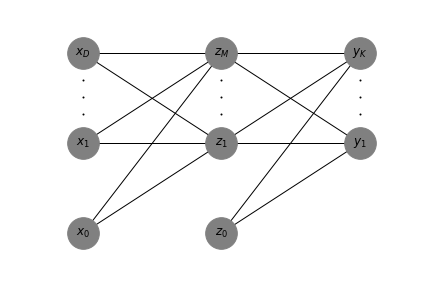
\includegraphics[scale=0.7]{Network.png}
\end{figure}

Equation 1 can easily be generalized by stacking more layers into the network, thus making it a multi-hidden-layer network. This is not in the scope of this thesis however.

\subsection{The activation function}
As touch upon in the previous Section, 2.1, $\widetilde{g}$ and $g$ in Equation 1 are activation functions. An activation function in ANN terminology is a function that defines how the output of a certain node will look like. An analogy would be the binary activation of a node in a computer circuit, which can be either $1$ or $0$. Indeed, if the binary function in Equation 2,

\begin{equation}
\hat{g}(a) = 
     \begin{cases}
       1 \ \text{if} \ a > 0 \\
       0 \ \text{otherwise} \\ 
     \end{cases}
\end{equation}

is used as activation in a zero hidden layer neural network, the ANN is called a \textit{Perceptron}.
\\

Another famous activation function is the sigmoidal function,

\begin{equation}
s(a) = \frac{1}{1 + e^{-a}}
\end{equation}

which when plotted forms the shape of an \textit{S}. Because of the geometrical shape of the sigmoidal activation function, it's derivative at small and large arguments is close to zero. This can yield a problem often called \textit{vanishing gradient}. The problem occurs because of the use of the chain rule in the backpropagation algorithm used to calculate the gradient (see Section 2.3).
\\

A popular alternative to the sigmoidal function has lately become the rectified linear unit, ReLU, function (Sonnoda \& Murata 2015),

\begin{equation}
    g(a) \equiv \max(0,a) \text{ and } g^{\prime}(a) =         \begin{cases}
            1 \text{ if } a > 0 \\
            0 \text{ otherwise}
        \end{cases}
\end{equation}

which solved the problem of \textit{vanishing gradient} because of its derivative.

\subsection{General derivation of backpropagation}

In order for a network to learn a suitable mapping from the input data to the output data it needs training. Network training consists of optimizing an error function with respect to the weights and biases. In order to optimize the error function, the gradient of the error function needs to be calculated. This is done by a method called backpropagation.
\\

In this section a derivation of backpropagation for a general feed forward network is given.
\\

Consider the following,

\begin{equation}
    a_j = \sum_{i} w_{ji}z_i + w_{j0}
\end{equation}

which describes a node in a general feed forward network, where $z_i$ is the activation of a node from the previous layer. $w_{j0}$ is the bias. Now, consider again a non-linear wrapping of $a_j$ by a differentiable function $g(\cdot)$,

\begin{equation}
    z_j = g(a_j)
\end{equation}

Note that some or all of $z_i$ could be input variables fed into the network, in which case they are denoted $x_i$. Note also that the units $a_j$ could be an output unit, in which case its activation is called $y_k$.
\\

Remember that the goal is to find suitable values for the weights and biases of the network. In order to do so an error function is needed to be defined,

\begin{equation}
    E = \sum_j^K E^{(j)}
\end{equation}

The error function is described by a sum since the output is a vector. Further it is assumed that $E^{(j)}$ is differentiable and can be written as a function of the output, $a_j$.

\begin{equation}
    E^{(j)} = E^{(j)}(a_1,...,a_c)
\end{equation}

Notice that the output from the network, $y_k$, is a function of the weights and biases, i.e. the adjustable parameters of the network. This means that $\^{E}$ can be defined as a function of $w$, $\^{E}(w) \coloneqq  E(a(w))$. With a little abuse of notation $\^{E}$ will now be referred to as $E$.
\\

Now consider differentiating the error function for a particular output, $E^{(j)}$, with respect to some weight, $w_{ji}$. Note that $E^{(j)}$ depends implicitly on $w_{ji}$ through $a_j$, see Equation 5, since $E^{(j)}$ is assumed to be a function of $a_j$. This means the chain rule can be utilized in order to split the derivative.

\begin{equation}
    \frac{\partial E^{(j)}}{\partial w_{ji}} = \frac{\partial E^{(j)}}{\partial a_j} \frac{\partial a_j}{\partial w_{ji}}
\end{equation}

Now the \textit{deltas}, also referred to as errors, are defined, i.e. the error from the above layer,

\begin{equation}
    \delta_j \equiv \frac{\partial E^{(j)}}{\partial a_j}
\end{equation}

Using Equation 5 the local derivative becomes,

\begin{equation}
    \frac{\partial a_j}{\partial w_{ji}} = z_i
\end{equation}

Substituting Equation 10 and 11 into 9,

\begin{equation}
    \frac{\partial E^{(j)}}{\partial w_{ji}} = \delta_j z_i
\end{equation}

One thing to note here is that Equation 12 has the same form as it would have if it were derived from a single layer network. Thus Equation 12 states that the derivative is obtained by multiplying the error, i.e. delta, which is the error calculated from the layer above, with the local derivative.
\\

Considering the output nodes, the activation in Equation 6 is now denoted $y_k$ and the following expression is formed,

\begin{equation}
    \delta_k \equiv \frac{\partial E^{(j)}}{\partial a_k} = g^\prime(a_k) \frac{\partial E^{(j)}}{\partial y_k}
\end{equation}

The derivatives for the hidden units needs also to be evaluated, the chain rule is used again,

\begin{equation}
    \delta_j \equiv \frac{\partial E^{(j)}}{\partial a_j} = \sum_k \frac{\partial E^{(j)}}{\partial a_k} \frac{\partial a_k}{\partial a_j}
\end{equation}

Now consider the following algorithm for backpropagation,

\begin{equation}
    \delta_j = g^\prime (a_j) \sum_k w_{kj} \delta_k
\end{equation}

One arrives at the backpropagation formula, i.e. Equation 15, by noticing that in Equation 14 the variation in $a_j$ goes though $a_k$ and by substituting Equation 10 into 14 and make use of Equation 5 and 6.
\\

This may seem complicated but the fact is that the $\delta$'s for the output units is known and therefore we can apply Equation 15 recursively on any feed forward network of given depth.
\\

Algorithm 1 is showing the backpropagation algorithm as pseudo code.
\\

\begin{algorithm}[H]
 %\KwData{this text}
 \KwResult{Matrix of gradients}
 initialization\;
 \While{Not First Layer of Weights + 1}{
    \For{each weight $w_i$ in layer}{
  %read current\;
      \eIf{Final Layer}{
       set $\delta_i = \frac{\delta E}{\delta a_i} g^\prime (a_i)$ \;
       }
       {
       set $\delta_i =  g^\prime (a_i) \sum_k w_{ki} \delta_k$ \;
      }
      save $\delta_i$ to Matrix
        }
 }
 \caption{Backpropagation pseudo code}
\end{algorithm}


\subsection{Network training with gradient descent}
Network training consists of minimizing the error function. In Section 2.3 a method of calculating the derivatives of the error function was presented – backpropagation. The error function is a function of the adaptive weights and biases of the network, which can be represented by a vector, \textbf{w}. Analytically one would like to find for which vector, \textbf{w}, such that, $\nabla E = 0$. Notice that this is an optimization problem of very high dimensionality, since the weight space is generally large.
\\

Backpropagation helps one to find the derivatives of the error function. Furthermore a method which finds the vector, \textbf{w}, that minimizes the error function is needed. One of the most common and simplest methods is \textit{gradient descent}.
\\

The gradient descent algorithm starts with an initial guess of the weight vector, $\textbf{w}^{(0)}$. It then evaluates the gradient of the error function, using backpropagation, at that point and moves the point in the opposite direction. I.e. at step $\tau$, the algorithm moves a point a short distance in the direction of the negative gradient, evaluated at $\textbf{w}^{\tau}$,

\begin{equation}
    \Delta \textbf{w}^{\tau} = - \alpha \nabla E \vert_{\textbf{w}^{\tau}}
\end{equation}

where $\alpha$ is the \textit{learning rate}.
\\

The basic version of the gradient descent method is indeed a target for the non-convexity trap, in which the algorithm converges to a minimum which is not the global as the objective function is not convex.

\subsection{Stochastic gradient descent}
Since the basic version of the gradient descent is not an optimal way of numerically optimizing, several slightly more advanced methods yielding significantly better results have been developed. SGD (stochastic gradient descent) is a family of methods which usually outperforms the basic method. The SGD methods calculate only a part of the gradient at each iteration.
\\

Suppose that the objective function that is about to be minimized is as Equation 7 in Section 2.3 \textit{General derivation of backpropagation},

\begin{equation}
    E = \sum_j^K E^{(j)}
\end{equation}

Instead of calculating the gradient of the full batch, i.e. of all $j's$, the gradient is calculated of a random subset. Hence, the SGD optimization is functioning the same way as the ordinary gradient descent with the difference that the gradient is calculated for a subset of the objective function. This yields a faster optimization.


\subsubsection{Adam optimizer}
Adam (adaptive moment estimation) is a SGD method introduced by Ba and Kingma (Ba \& Kingma 2015). The Adam algorithm updates the gradient in each step based on a momentum method. The method calculates dynamical learning rates for each time step based on the first, $m_t$, and second, $v_t$, moments of the gradient, i.e. the mean and the uncentered variance of the gradient.
\\

Algorithm 2 is showing the Adam algorithm (Ba $\&$ Kingma 2015).
\newpage

$g_t^2$ indicates the elementwise square $g_t \circ g_t$. Good default settings for the tested machine learning problems are $\alpha = 0.001$, $\beta_1 = 0.9$, $\beta_2 = 0.999$ and $\epsilon = 10^{-8}$. All operations on vectors are element wise. With $\beta_1^t$ and $\beta_2^t$ we denote $\beta_1$ and $\beta_2$ to the power t.
\\

\begin{algorithm}[H]
 
 \textbf{Require:} $\alpha$: Stepsize.
 \\
 \textbf{Require:} $\beta_1$, $\beta_2$ $\in$ [0,1): Exponential decay rates for the moment estimates.
 \\
 \textbf{Require:} $E(w)$: Stochastic objective function with parameter $w$.
 \\
 \textbf{Require:} $w_0$: Initial parameter vector.
 \\
 $m_0 \leftarrow 0$ (Initialize $1^{st}$ moment vector).
 \\
 $v_0 \leftarrow 0$ (Initialize $2^{st}$ moment vector).
 \\
 $t \leftarrow 0$ (Initialize timestep).
 %\KwData{this text}
 %\KwResult{$\theta_t$ (Resulting parameters)}

 %initialization\;
 \While{$w_t$ not converged}{
    $t \leftarrow t+1$
    \\
    $g_t \leftarrow \nabla_{w} E_t(w_{t-1})$ (Get gradient w.r.t stochastic objective at timestep t)
    \\
    $m_t \leftarrow \beta_1 \cdot m_{t-1} + (1-\beta_1) \cdot g_t$ (Update biased first moment estimate)
    \\
    $v_t \leftarrow \beta_2 \cdot v_{t-1} + (1-\beta_2) \cdot g_t^2$ (Update biased second moment estimate)
    \\
    $\hat{m}_t \leftarrow m_t / (1 - \beta^t_1)$ (Compute bias-corrected first moment estimate)
    \\
    $\hat{v}_t \leftarrow v_t / (1 - \beta^t_2)$ (Compute bias-corrected second raw moment estimate)
    \\
    $w_t \leftarrow w_{t-1} - \alpha \cdot \hat{m}_t / (\sqrt{\hat{v}_t}+ \epsilon)$
 }

 \KwResult{$w_t$ (Resulting parameters)}
 
 \caption{Adam optimization pseudo code}
\end{algorithm}
\vspace{0.5cm}

An important implication of the Adam algorithm is its adaptive learning rate. Consider the last line in the pseudo code of \textit{Algorithm 2}, also assume $\epsilon = 0$. The rate at which the parameters are updated at time $t$ becomes,

\begin{equation}
    \Delta t = \alpha \cdot \hat{m}_t / \sqrt{\hat{v}_t}
\end{equation}

\newpage

\subsection{Universal approximation theorem}
One of the most classic theorems within the mathematics of neural networks is the \textit{universal approximation theorem}. The theorem states that a feed forward network with one hidden layer and a finite number of nodes can approximate arbitrary well any continuous map from one finite-dimensional space to another. One of the first papers investigating the universal approximation properties is \textit{Approximation by superpositions of a sigmoidal function} (Cybenko 1989). Cybenko proved the theorem for the sigmoid activation function. Hornik later showed that the theorem is not limited by the sigmoidal activation function and proved the theorem for an arbitrary activation function under some assumptions (Hornik 1991).
\\

A version of the theorem is stated in \textit{Neural networks: a comprehensive foundation} (Haykin 1998),

\newtheorem*{mydef}{Universal approximation theorem}

\begin{mydef}
Let $g (\cdot)$ be a nonconstant, bounded, and monotone-increasing continuous function. Let $I_{D}$ denote the $D$-dimensional unit hypercube $[0,1]^{D}$. The space of continuous functions on $I_{D}$ is denoted by $C(I_{D})$. Then, for all $f \in C(I_{D})$ and $\epsilon > 0$, there exist an integer $M$ and sets of real constants, $\{w_j^{(2)}, w_{ji}^{(1)}, w_{j0}^{(1)} \mid i = 1,\ldots ,D \ \textit{and} \ j = 1, \ldots\ , M \}$ such that the approximate realization of $f(\cdot)$

\begin{equation}
    F(x_1, ..., x_{D}) = \sum_{j=1}^{M} w^{(2)}_{j} g \left( \sum_{i=1}^{D} w_{ji}^{(1)} x_i + w^{(1)}_{j0} \right)
\end{equation}

satisfies

\begin{equation}
    \vert F(x_1, ..., x_{D}) - f(x_1, ..., x_{D}) \vert < \epsilon
\end{equation}

for all $(x_1, x_2, ..., x_{D}) \in I_{D}$.

\end{mydef}

Note that Equation 19 is in fact a variant of Equation 1, which means that it is a one hidden layer neural network with $D$ input nodes and $M$ hidden nodes. Furthermore, in this version of the theorem the activation function is assumed to be nonconstant, bounded, and monotone-increasing. Thus, the logistic function and the sigmoid function are e.g. meeting these assumptions, however the ReLU function is not since it is in fact unbounded.
\\

Sonoda and Murata investigated the universal approximation theorem with respect to the ReLU activation function (Sonoda \& Murata 2015). The main reason for this was that the ReLU function is the new standard for deep learning. In their paper they showed that a neural network with ReLU activation function still satisfies the universal approximation property.

\section{The Error Surface}
It is common to refer to the graph of the error function $E(w)$ as the error surface. In this section some properties of the error function and the error surface is discussed.
\\

The error function of neural networks is non-convex (Lipton 2016). As a result one can not guarantee that any local minimum found during optimization is a global minimum. This transforms the training of a neural network into a complicated problem as one can never guarantee that a found value for the error function is any close to a global minimum. This is further amplified by the fact that the error function is often incredibly high dimensional. If one looks at the error function, $E(w)$ Section 2.3, one sees that the dimensionality of the error surface is directly correlated with the number of weights in the network.
\\

\subsection{Features of the error surface in relation to the size of the network}
Choromanska et al. did extensive analysis on how the error surface of neural networks looks like. Three important features can be directly extracted from the report (Choromanska et al. 2015),
\begin{enumerate}
\item "For large-size networks most local minimas are equivalent and yield similar performance on a test set."
\\

\item "The probability of finding a 'bad' (high value) local minimum is non-zero for small-size networks and decreases quickly with network size."
\\

\item "Struggling to find the global minimum on the training set (as opposed to one of the many good local ones) is not useful in practice and may lead to over fitting." (Choromanska et al. 2015).
\end{enumerate}
\vspace{0.5cm}

What this implies is that, it is generally better to opt for a larger network when trying to train a neural network, as the probability of the training algorithm to get stuck in a bad local minimum decreases with network size. However one has to be wary of over fitting when training larger networks. Over fitting is further discussed in Section 4.1 and 4.2.
\\

However, any good value on an error function might not be any of these good valued local minimum. It might be the case that the optimization algorithm has reached a bad valued plateau. That is a large area on the error surface which is seemingly flat (Dauphin et al. 2014). This emphasizes the importance of having a good update rule such as the Adam-optimizer discussed in Section 2.5.1, as it might help the algorithm to traverse the plateau in a reasonable amount of time. If the algorithm does not take sensible step sizes to get away from the plateau, the training algorithm might perform all of its iterations or be lead to believe that it has reached a minimum, without even leaving the plateau. Thus leaving the value of the error higher than it could potentially be and as a result, negatively impact the networks performance after training. 
\\

Another way to tackle the problem of bad plateaus, and bad local minima in small networks even, is to initialize the neural network with different initial weights when one retrains it due to poor performance, as the network might by luck, avoid the bad valued areas on the error surface altogether.

\section{Training networks is hard}
In most real world applications of neural networks one wants to predict some out-of-sample result, based on an in-sample data. In the scope of this thesis only in-sample approximation is considered as more emphasis is put onto the mathematical structure of the feed forward neural network as opposed to any real world application. However, this section will be treating neural networks used for predicting out-of-sample data as it sheds light on some interesting problems regarding data driven prediction in general and how one generally solves these problems when they arise regarding neural networks.
\\

As discussed in Section 3 one generally needs a somewhat large amount of nodes to solve any non trivial problem, due to the properties of the error function. That is, maybe a solution to a specific problem can be constructed with a neural network using the right weights, biases and some number of nodes. However, as the proper values for the weights and biases are not known beforehand, they have to be found using the training algorithm. Even though a good local minimum might exist, the network can still get stuck in some bad local minimum during training. Due to the fact that fewer nodes reduces the dimensionality of the error function. This means that the training algorithm is unable to find suitable values for the weights and biases and thus the error may remain high in any measure.
\\

The obvious solution to this problem is to provide the network with more degrees of freedom. In the case of a general neural network that means more layers and nodes. In the case of the single layer feed forward network more nodes. As is discussed in Section 6 giving the single hidden layer feed forward neural network with ReLU activation units more nodes is equivalent to increasing the potential number of knots in a linear spline. This way one can see that increasing the number of hidden nodes increases the expressibility of the neural network as the approximation can more accurately model more complex functions.
\\

This is good for in-sample approximations but can lead to a problem called over fitting when doing out-of-sample predictions.

\subsection{Cross Validation}
One way to evaluate how well a model might predict out-of-sample, is to split the data set used to train the network into two sets, a training set and a validation set. The ratio between these sets varies but generally the validation set is smaller than the training set. The model is then trained on the training set, and then has its accuracy validated on the validation set.
\\

The reasoning to do this split is that the network can use one part of the data set to learn some generalisation of the underlying distribution of the data set as a whole and the other set to validate that it is learning a generalisation that might be good to predict out-of-sample. Basically what one tries to achieve is some sort of simulation of out-of-sample prediction using the validation set.
\\

It is important that the split of the data set is done randomly, as the underlying distribution of the whole data set has to be preserved both in the training set and the validation set.

\subsection{Over fitting}
If an approximation of a function has too many free variables it can be over fitted to the data. That is the approximation follows the data points so closely, that out-of-sample predictions become bad.
\\

This can be illustrated, see Figure 2, using polynomial regression. In the following example ten equally distant data points in the range $x_i\in[1,10]$ are mapped to the function $y(x) = x + N(0,0.4)$, where $N(\mu,\sigma)$ is the normal distribution. One would expect the value of $y(11)$ to be $11 \pm 0.4$. A decent approximation for this can thus be constructed using polynomial regression of degree $1$. However if one approximates the function using a polynomial interpolation of degree $6$. The out-of-sample prediction becomes very incorrect.
\\
\begin{figure}[h]
\centering
\begin{subfigure}{0.5\textwidth}
  \centering
  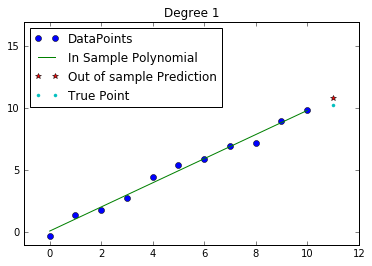
\includegraphics[width=1\linewidth]{overfit1.png}
  \caption{Degree 1 Prediction}
  \label{fig:sub1}
\end{subfigure}%
\begin{subfigure}{.5\textwidth}
  \centering
  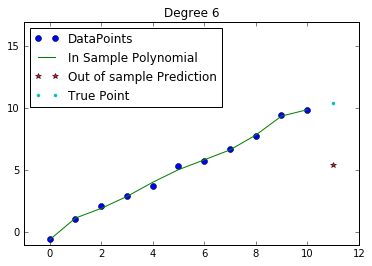
\includegraphics[width=1\linewidth]{overfit2.png}
  \caption{Degree 6 Prediction}
  \label{fig:sub2}
\end{subfigure}
\caption{Plots of Polynomial interpolation of two different degrees}
\label{fig:test}
\end{figure}

Even though the second interpolation has more free variables to adjust, in order to solve the problem at hand, the prediction became worse. The same principle applies to neural networks. More nodes does not necessarily mean a better out-of-sample prediction.

\subsection{Methods to combat over fitting}
As stated before neural networks are prone to over fit as they generally contain more free variables than is necessary to directly solve a problem, as it is hard to train them otherwise. The result is that various techniques to combat over fitting has been developed. What follows is a description of some of the most common and effective method to combat over fitting.

\subsubsection{Early stopping}
If one suspects that the models accuracy has stopped improving one can simply stop the training of the network. One way to detect this is to measure whether the error of the validation set has converged with some threshold. If the validation error indeed has stopped improving this can be an indication that the network is starting to over fit to the training data.

\subsubsection{Regularization}
Another way to hinder over fitting is to regularize the error term used in the backpropagation algorithm (Bishop 2006). That is, one tries to punish over generalization while still keeping the expressibility of the neural network high.
\\

This is achieved by adding some penalizing term to the error function thus reducing the smoothness of the curve produced by the neural network. As seen in the polynomial interpolation example above a too high degree of smoothness can be devastating for out-of-sample predictions.
\\

One example of a regularization term is the $L2$ term defined as,
\begin{equation}
L2 = \frac{\lambda}{2} \sum_w w^2
\end{equation}
where $w$ are the weights of the network. $\lambda$ is a constant the adjusts how aggressively the regularization term affects the error.
\\

This term is then simply added to the error function as following
\begin{equation}
E(w) = \sum_j^K E^{(j)} + L2
\end{equation}
The intuition behind this kind of regularization is that it punishes the network for learning weights that have too large values. Thus if a weight is to receive a large value it has to considerably increase the accuracy for the network. This helps keeping the degree of smoothness lower as the likelihood that one single weight becomes too large is diminished.
\\

The $L2$ is just one example of a regularization term. There are several different regularization terms good for different scenarios depending on the specific problem.
\\

Another regularization technique is called dropout (Srivastava 2014). Every time a feed forward propagation is started some portion of the inner nodes in the network are disabled. The ratio varies but something like $50\%$ of the nodes being disabled is not uncommon.
\\

This also helps reduce over fitting as the network has to be able to solve the problem at hand over several subset of nodes. That is, it can not rely on one single subset of its nodes in order to solve some specific problem or input. Therefore it has to spread its generalization more across the whole of the network.
\\

The problem with having an expressive network, that is a network with many inner nodes, is that eventually the network might become a so called "glorified lookup table". That is more or less each node in the network has learned to correspond to a certain input. This produces good accuracy on the training set but bad accuracy on the out-of-sample predictions. If nodes are disabled at random this might prevent the network to over fit.
\subsubsection{Reduce the size of the network}
One last method presented here is simply to reduce the size of the network. If the problem is simply that the network is too expressive one can reduce the number of hidden nodes in the network. The high degree of expressibility might be what allows the network to generalise the problem at hand, but if it can achieve the same task with fewer nodes over fitting could be reduced by decreasing the number of hidden nodes.

\newpage

\section{The ReLU network model}
The neural network model that will be investigated in this thesis is a network with one single hidden layer, with an arbitrary number of nodes, and the rectified linear unit as activation function for the hidden layer and the unit function as final layer. The network maps one input value to one output value. Hence, $y: \mathbb{R} \rightarrow \mathbb{R}$. Thus the network can be expressed as:

\begin{equation}
    y = \sum_{i=1}^n w_i^{(2)} z_i + b^{(2)}
\end{equation}

where,
\begin{equation}
    z_i = g(w_i^{(1)}x + b_i^{(1)})
\end{equation}
\\

Figure 3 is a visual representation of Equation 23 and Equation 24.

\begin{figure}[H]
\caption{Feed forward network mapping one input to one output.}
\centering
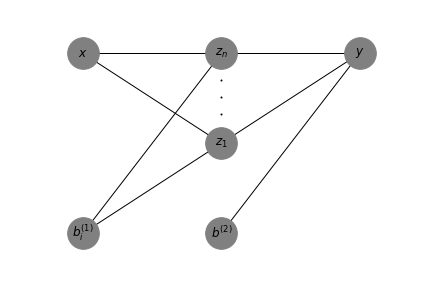
\includegraphics[scale=0.7]{Network2.png}
\end{figure}


\subsection{ReLU activation function}
The ReLU (rectified linear unit) function has become a widely used and popular activation function within neural networks, especially deep neural networks. In the beginning researchers were inspired to use ReLU activation function because of its biological similarity. Later the function showed empirical improvements in training speed of neural network and good results. One explanation why the ReLU function might yield great out-of-sample predictions is due to its simplicity. Another documented reason for increased performance is the functions derivative. The derivative is easily computed and does not suffer from the problem of vanishing gradient. Vanishing gradient is a problem that occurs if sufficiently many derivatives close to zero are multiplied together due to backpropagation. The famous sigmoidial activation function experiences this problem.
\\

The ReLU function is defined as follows,

\begin{equation}
    g(a) \equiv \max(0,a) \text{ and } g^{\prime}(a) =         \begin{cases}
            1 \text{ if } a > 0 \\
            0 \text{ otherwise}
        \end{cases}
\end{equation}

Notice that the derivative of the ReLU function is analytically solvable, which makes the function easy to use as an activation function in a neural network.


\section{Theoretical Results}
\subsection{ReLU nets are splines}
One curious property of feed forward networks with ReLU activation functions in their hidden layers is that they are equivalent to linear splines. The theoretical results in this thesis is inspired by Chen's paper \textit{The upper bound on knots in neural networks} (Chen 2016).
\\

In order to show that the ReLU net is a linear spline it is helpful to first define what a linear spline is.

\newtheorem*{mydef3}{Definition of linear spline}
\begin{mydef3}
A function, $S$, is called a \textit{linear spline} or a \textit{spline of degree 1} if for a finite set of knots $x_0,x_1,...,x_n$ the following two conditions hold
\begin{enumerate}
    \item on each interval $[x_{i-1},x_i]$, $S$ is a polynomial of maximal degree $1$
    \item $S$ is continuous
\end{enumerate}
\end{mydef3}

\newtheorem*{mydef4}{Theorem (1): Single hidden layer neural networks with ReLU activation functions are linear splines}
\begin{mydef4}
Let $y$ be a neural network defined by Equation 23 and 24 with the ReLU activation function defined as in Equation 25. $y$ is a function  $\mathbb{R} \rightarrow \mathbb{R}$ satisfying the conditions in the definition of the linear spline and is thus a linear spline. The knots are defined by the networks's weights and biases.
\end{mydef4}

Proof: 
\begin{enumerate}
\item Let g(a) be the ReLU function. g(a) is a linear spline with knots $X = \{ a_{min}, 0, a_{max} \} $
\item Let z be an inner node of the neural network $y$ defined as $z = g(wx + b)$. z is a linear spline with knots $X = \{\frac{x_{min} - b}{w}, \frac{-b}{w}, \frac{x_{max} - b}{w} \} $
\item The whole network $y$ is an affine transformation of the inner network nodes $z_1,z_2,...,z_n$ Such that: $y(x) = w^{(2)}_1g(w_1^{(1)} x + b^{(1)}_1) + w^{(2)}_2g(w_2^{(1)} x + b^{(1)}_2) + ... + w^{(2)}_n g(w_n^{(1)} x + b^{(1)}_n) + b^{(2)}$.
\end{enumerate}
\vspace{0.3cm}

By creating the set of knots $X_y$ for $y$ as the union of all the knots of the inner network nodes, $X_1,X_2,...,X_n$ such that: $X_y = X_1 \cup X_2 \cup ... \cup X_n$. Then $y$ is defined by a set of knots. As y consists of a linear combination of $z_i$'s the two conditions for linear splines are preserved in $y$. Combining these results one sees that $y$ is a linear spline. $\qed$



\subsection{Upper bound of knots in one layer network}
\newtheorem*{mydef8}{Theorem (2): The number of inner spline knots is bounded by the number of inner network nodes}
\begin{mydef8}
The number of inner knots, $k$, of a spline, $y$, defined by Equation 23 and 24 with activation function as defined in Equation 25, is bounded by the number of inner network nodes, $n$. That is, the number of inner spline knots satisfies the relation $k \leq n$.
\end{mydef8}

Proof: Writing Equation 23 as $y = w_1^{(2)} z_1 + w_2^{(2)} z_2 + ... + w_n^{(2)} z_n + b^{(2)} $, where $z_i$ is defined as in Equation 24. The derivative of $y$ with regard to $x$ is,  $y^\prime=w_1^{(2)} z_1^\prime w_1^{(1)} +...+ w_n^{(2)} z_n^\prime w_1n^{(1)}$. The derivative consists of $n$ terms $z_1,z_2,...z_n$. The terms can at most be discontinuous at one point. That is when the argument for $z_i(x)$ is $x = \frac{-b_i^{(1)}}{w_i^{(1)}}$. Hence, there are at most $n$ discontinuities in $y^\prime$.
\\

The relation is $k \leq n$ due to the fact that two knots can overlap one another if $(\frac{-b_i^{(1)}}{w_i^{(1)}}) = (\frac{-b_j^{(1)}}{w_j^{(1)}})$ for two different network nodes $z_i$ and $z_j$ The knots can also lie outside of the range of $[x_{min},x_{max}]$ if  $\frac{-b_i^{(1)}}{w_i^{(1)}} < x_{min}$ or $\frac{-b_i^{(1)}}{w_i^{(1)}} > x_{max}$ $\qed$
\\

Using Theorem 1 one can see that if two or more of the $n$ terms $y^\prime$ have their discontinuity at the same position their knots will coincide. That is if $\frac{b_i^{(1)}}{w_i^{(1)}} = \frac{b_k^{(1)}}{w_k^{(1)}}$ happens to coincide for the two network nodes $z_i$ and $z_k$. If $w^{(1)}_i$ also is small or if $b^{(1)}_i$ is large the knots might lie outside of the set of knots $X$ as this set is bounded. Since $y$ is defined in a finite interval then that knot will not exist for $y$ as it is defined by its knots.

\newpage

\section{Spline interpolation}
In Section 8, \textit{numerical experiments}, a neural network with one hidden layer and the ReLU activation function is compared to a linear interpolating spline with equidistant placed knots. This section will give a short overview of spline interpolation (Süli \& Mayers 2003) (Powell 1981). In Section 6, \textit{Theoretical results}, the definition of a linear spline is stated and it is shown that the ReLU network is a spline, however it is not an interpolating spline by definition.
\\

The word \textit{interpolate} means simply to put something in between other things. In numerical analysis interpolation is used to estimate values between known values. Given some points, $\{x_0,...,x_n\}$, a function $f$ is interpolating another function $g$ at the given points if $f(x_i) = g(x_i)$ at those points. There are several ways to find functions that share the same value as the function one wants to interpolate, although polynomial interpolation of different degrees is common.
\\

Linear spline interpolation builds upon the idea of polynomial interpolation of degree one, i.e. linear functions, that are piecewise defined. An example of equidistant linear spline interpolation would be if one has some equidistant placed points  $\{x_0,...,x_n\}$ and one connects these points with lines, then the piecewise defined linear function that connects these points is a linear spline.


\section{Numerical Experiments}
In this section the theoretical results from the previous section will be demonstrated. It will be shown by example that feed forward neural networks with one hidden layer are equivalent to some linear spline with some set of knots. The network will be compared to a linear spline constructed using interpolation with equidistant knots. This is done so that their errors can be compared. The network will also be plotted with the knots marked as red lines. This is done to illustrate the property that the number of inner knots is bound by the number of network nodes.
\\


An artificial neural network with an upper bound on the number of knots, $k \leq n$, is compared to a linear spline with $n$ knots. That is, the network will have at most as many knots as the linear spline function it will be compared to. The task is to approximate Runge's function,

\begin{equation}
    \frac{1}{1+25x^2}, \ \ \ x \in [-1, 1]
\end{equation}

Runge's function is famous from \textit{Runge's phenomenon}. The phenomenon appears when one tries to interpolate Runge's function. Oscillation is created at the beginning and end of the interval, $[-1,1]$, when the degree of the interpolating polynomial is increased. The interpolation inconvenience can be adjusted by instead using splines. However, the problem of choosing the position of the knots is still present. An usual methodology is to use equidistant knots, although this is usually not the optimal choice but depends on the function one tries to approximate. As was shown in Section 6, the neural networks investigated in this thesis are splines, the inner knots are present at the points $\frac{-b_i}{w_i}$, also shown in the theoretical results Section 6. The weights and biases of the networks are adjustable parameters decided by the training of the network, hence the placement of the knots is decided in the optimization of the weight-space of the network. To measure accuracy of the approximation the mean-squared-error function, $MSE = \frac{1}{n} \sum_{i=1}^n (\hat{y}_i - y_i)^2$, was used.

\subsection{Instructions of how the approximation, using neural networks, was performed.}
Thanks to the \textit{Universal Approximation Theorem} discussed in Section 2.6 it was known that a single hidden layer neural network with ReLU-activation units in the hidden layer and linear activation units in the output layer was potentially sufficient to find an arbitrary good approximation for Runge's function.
\\

To realise the network, Google's computational library \textit{TensorFlow} was used. TensorFlow comes with a Python wrapper and thus one can write TensorFlow code in the Python language. An API called Keras which is written over TensorFlow was also used as the API provides powerful and easy to use tools for working with artificial neural networks. What follows is a short instruction on the program that was written in order to realise the numerical approximation of the Runge's function. In addition to Keras and TensorFlow the Python library Numpy was also used, as it offers tools for working with mathematical objects in the Python language.
\\

First of: a simple Python function which generated a Sequential() object from the Keras models package with a variable number of hidden layers with ReLU activation function was written. 
\begin{lstlisting}
model = createNetwork(NoHiddenNodes)
\end{lstlisting}
This way: model is a TensorFlow computational graph which represents the neural network discussed in this thesis. The parameter 'NoHiddenNodes' allows one to change how many hidden nodes the model contains.
\\

To generate data for the training a list of $10000$ elements in the range $[-1,1]$ was generated using Numpy in the following way.
\begin{lstlisting}
x = np.random.rand(1000,1)*2
x = x-1
\end{lstlisting}
All of these values was mapped to Runge's function.
\begin{lstlisting}
runge = lambda x: (1/(1+25*x**2))
y = runge(x)
\end{lstlisting}
After that, the network was trained to be able to approximate Runge's function. Here Keras offers a myriad of tools to realise the training. First of the "Adam" optimizer was used. The learning rate was set to $lr = 0.0001$. Different parameters were tested but it was settled on this learning rate as it worked well. One could probably speed up convergence if one were to investigate a more optimal learning rate. The optimizer is created in Keras as following:
\begin{lstlisting}
adam = keras.optimizer.adam(lr=0.0001)
\end{lstlisting}
In order to speed up the training between different variations of networks "EarlyStopping" from the keras package callbacks was used. That is, if the error of the validation set stops improving the training stops. The early stopping was configured to listen to the MSE value for the validation set after each epoch. If the value of the MSE had not improved in the last two epochs training was stopped and the model was returned. This looks like the following in code:
\begin{lstlisting}
early_stopping = EarlyStopping(monitor='val_loss',patience=2)
\end{lstlisting}
'monitor' is which error the EarlyStopping listens to. 'Patience' is how many epochs the EarlyStopping is waiting before stopping the training.
\\

One has to compile the model object before it can be trained.
\begin{lstlisting}
model.compile(loss ='mean_squared_error', optimizer=adam)
\end{lstlisting}
Finally the network is trained in the following piece of code:
\begin{lstlisting}
model.fit(x, y, nb_epoch=50000, batch_size=8000, verbose=1,validation_split=0.2,callbacks=[early_stopping])
\end{lstlisting}
The parameter 'x' is the list of values containing $10000$ random elements in the range $[-1,1]$. The parameter 'y' is the $10000$ corresponding values from Runge's function.
\\

One has to settle on a number of epochs that the network should iterate over before it stops the training. As early stopping was used a very high number of epochs was chosen. In none of the many trainings that was performed did the various networks ever reach $50000$ epochs before the EarlyStopping fired.
\\

As the data was very simple in this application the whole batch was fed into the network at the same time. That is: 'batchsize' $= 8000$. The reason that 'batchsize' was not set to $10000$ was that $2000$ of the elements was used in the validation set. This was determined by the parameter 'validationsplit' $=0.2$.
\\

Finally 'verbose' was set to 1 as this provided some information about how the training is performing in the console of the Python program. EarlyStopping was also passed as an argument so that the training had the ability to stop early if the validation error stopped improving.
\\

When the training was done the approximation of Runge's function was retrieved from model in the following way. Some random data was created in the interval $x\in[-1,1]$ sampled from the normal distribution with mean $0$ used for testing the function.
\begin{lstlisting}
approximation = model.predict(np.sort(x, axis=0))
\end{lstlisting}
'approximation' is now a NumPy array containing the predicted function values.
\\

The numerical approximation constructed by the neural networks was also compared to a linear spline using equidistant knots. This was done using the Python library SciPy, using the module "Interpolate".
\\

The two different approximations were plotted over Runge's function. The MSE for both approximations was compared in all the cases. What follows below are a few selected examples. In the column to the left the approximations are compared. In the column to the right the network approximation is plotted with its corresponding knots inside the domain $x_i\in[-1,1]$, using the formulae devised to calculate the position of the knots in Section 6.1, $x_i = \frac{-b_i}{w_i}$.
\\

Figure 4 shows three different networks compared to three different linear interpolating splines with equidistant knots. Figure 4 (A) shows a network with 2 nodes, yielding 2 inner knots, and 4 in total including the end points. It is plotted together with a interpolating linear spline that also exhibits 2 inner knots and 4 in total including the end points. One can see that the error of the network is $0.0110$ while the error for the linear spline is $0.0633$. In Figure 4 (B) the network is plotted together with lines showing the position of the knots. The same structure follows the rest of the plots in Figure 4.

\begin{figure}[H]
    \centering
    \begin{subfigure}{.45\textwidth}
        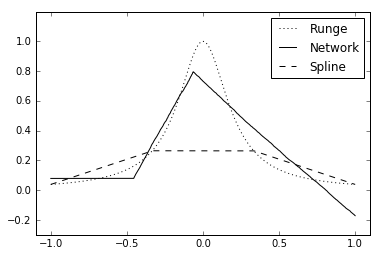
\includegraphics[width=\textwidth]{2nodes1.png}
        \caption{2 nodes}
        %\label{fig:subfig1}
        	\begin{tablenotes}
                 \tiny
            	\item  MSE spline: 0.0633. MSE network: 0.0110.
        	\end{tablenotes}
    \end{subfigure}
    \quad
    \begin{subfigure}{.45\textwidth}
        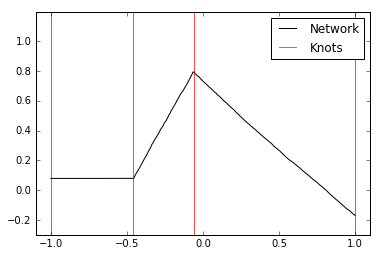
\includegraphics[width=\textwidth]{2nodes2.png}
        \caption{2 nodes: Location of knots}
        %\label{fig:subfig2}
    \end{subfigure}
    
    \begin{subfigure}{.45\textwidth}
        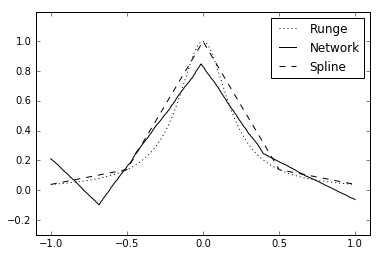
\includegraphics[width=\textwidth]{3nodes1.png}
        \caption{3 nodes}
        %\label{fig:subfig3}
            \begin{tablenotes}
                 \tiny
            	\item  MSE spline: 0.0070. MSE network: 0.0079.
        	\end{tablenotes}
    \end{subfigure}
    \quad
    \begin{subfigure}{.45\textwidth}
        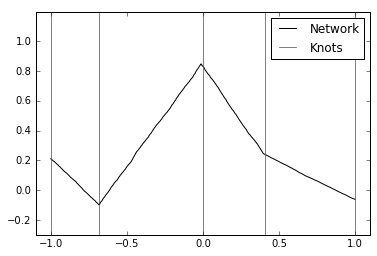
\includegraphics[width=\textwidth]{3nodes2.png}
        \caption{3 nodes: Location of knots}
        %\label{fig:subfig3}
    \end{subfigure}

    \begin{subfigure}{.45\textwidth}
        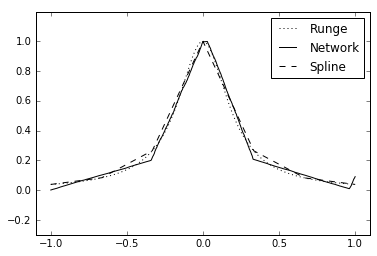
\includegraphics[width=\textwidth]{5nodes1.png}
        \caption{5 nodes}
        %\label{fig:subfig3}
            \begin{tablenotes}
                 \tiny
            	\item  MSE spline: 0.0008. MSE network: 0.0007.
        	\end{tablenotes}
    \end{subfigure}
    \quad
    \begin{subfigure}{.45\textwidth}
        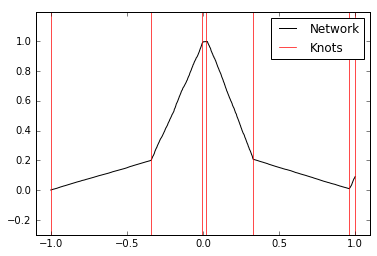
\includegraphics[width=\textwidth]{5nodes2.png}
        \caption{5 nodes: Location of knots}
        %\label{fig:subfig3}
    \end{subfigure}
\caption{Runge's Function, Interpolating Spline and Neural Network.}
%\label{3figs}
\end{figure}

\newpage

\section{Discussion}
\begin{itemize}
\item How does a single layer ANN with ReLU activation function approximate a function?
\end{itemize}
\vspace{0.5cm}

As shown in this thesis a neural network with a single hidden layer with ReLU activation is a linear spline. Thus the approximating function is built up by piece wise linear functions, as e.g. shown in Figure 4. This can explain one of the reasons why the ReLU function is such a popular activation function, and performs well. In Section 4.1 and 4.2 over fitting was discussed and an example with polynomial interpolation was given (Figure 2). If the approximating function has a too high sensitivity and over fits to the training data, one is exposed to the risk of bad out of sample prediction. Since it is shown that ReLU approximates with piece wise defined linear functions it is the least sensitive function in the family of polynomial splines.
\\

\begin{itemize}
\item How is a single layer ANN with ReLU activation function related to approximation theory?
\end{itemize}
\vspace{0.5cm}

In approximation theory splines and spline interpolation is commonly studied and since ReLU networks are essentially splines the two areas intersect. However, the statement that ReLU networks are splines doesn't necessarily make them interpolating splines. The definition of interpolation is nowhere to be found when we are defining the ReLU neural network. Instead the networks knots are placed using a training algorithm, trying to minimize some error.
\\

\begin{itemize}
\item How does the approximation change when adding or subtracting nodes?
\end{itemize}
\vspace{0.5cm}

Theorem 2 states that the number of knots of the linear spline is bounded by the number of inner nodes of the network. By adding a node/neuron into the neural network one is adding one degree of freedom to the network which makes it possible, although not a must, for the network to create one more knot to the spline. The reason why one more knot is not automatically created is because knots can intersect. As stated in the proof of Theorem 2, $(\frac{-b_i^{(1)}}{w_i^{(1)}})$ could happen to be equal to $(\frac{-b_j^{(1)}}{w_j^{(1)}})$, for two different network nodes $z_i$ and $z_j$, in this situation one more knot would not be added to the linear spline although one more inner node was added to the network. When subtracting an inner node from the ANN one reduces the maximum number of knots of the spline by one.
\\

\begin{itemize}
\item How does the approximation of a continuous function with the ReLU ANN compared to an interpolating linear spline with equidistant spaced knots?
\end{itemize}
\vspace{0.5cm}

As discussed in the thesis the position of the knots of the spline created by the neural network is decided by the weights and the biases of the neural network. This means that the positioning of the knots are part of the optimization problem. When the error function is minimized the adjustable parameters are changed, hence the weights and biases are changed, hence the positions of the knots are changed. An interpolating spline with equidistant placed knots has no flexibility in the position of the knots but to have them placed with equal distance. Furthermore, the interpolation has the constraint of being equal to the function it interpolates at a certain point, this does not apply to the neural network.


\section{Concluding remarks}
The ReLU activation function has been used successfully within neural networks during the last years. When looking at the simple hinge function it is not clear how it helps the network model to approximate anything at all. With some imagination one slowly starts to understand the connection to linear splines and how the mechanisms work. In the fast paced environment one lives in today it is easy to interpret machine learning and neural network theory as much more of a trial and error subject than a science. Data scientists might use algorithms and methods without exactly knowing how they work, as long as they perform well in the moment. For these reasons it has been delightful to investigate how a popular activation function, such as the ReLU function, actually helps the networks to approximate functions. If results like these are further investigated for other activation functions and other types of neural networks the field will more easily be understood by non-machine learning engineers, such as mathematicians, which could help the field of neural networks to continue improving.
\\

Apart from the sources referenced in this thesis there is some other noteworthy material to read regarding neural networks. The feed forward neural network discussed in this thesis is in a way the most simple of the neural networks. There are two other common types of neural networks that are important today, the \textit{convolutional neural network} and the \textit{recurrent neural network}.
\\

The convolutional neural network (Krizhevsky et al. 2012) is simply a deep feed forward neural network but it also contains convolutional and pooling layers. That is, the input is fed into a layer that applies a convolution operation to the input before passing it forward. This is done for a variable amount of layers before the data is passed into a pooling layer, which reduces the dimensionality of the data using some stride. A stride of say $2$ means that the pooling layer takes $2x2$ neighbouring data points in the data matrix and down samples it into a single data point. This can be done using something like the largest value in each stride or an average of the values in the stride. The down sampled data is then further fed into a variable amount of convolutional/pooling layers, heavily dependent on the problem at hand. When the convolutional/pooling phase of the feed forward propagation is over the data is fed into one or several layers of feed forward fully connected layers. After that back propagation can be applied to the network with respect to some sensible error function. What the convolutional nerual network allows one to do is to take something like a picture, find various edges and shapes in the picture and then analyse them using a deep feed forward network. These kind of networks have been very successful regarding image processing and convolutional neural network have been deployed in many applications where out-of-sample prediction regarding data like pictures is necessary.
\\

Recurrent artificial neural networks are a class of neural network that are related to autoregressive functions, in e.g. time series analysis, where $y_t$ depends upon $y_{t-1}$. An example of a structure of a recurrent networks could be, after data has been processed by a node it is not send forward in the network but again reprocessed by that node. One can think of recurrent neural networks have a feedback loop. There are several types of recurrent neural networks depending on the structure of the network. A common and popular recurrent network type is LSTM (long short-term memory) networks (Hochreiter \& Schmidhuber 1997). The LSTM networks consist not of nodes but of LSTM blocks and has \textit{memory}, that is the output of the network can depend on structures lagged in time. These LSTM networks can in fact store arbitrary long autoregressive structures. The recurrent networks, LSTM included, are often used for language processing and time series analysis.


\newpage

\section{References}
Adadi. M., Google Research et al. (2015). TensorFlow: Large-Scale Machine Learning on Heterogeneous Distributed Systems. Preliminary White paper, November 9, 2015.
\\

Ba L. J., Kingma P. D. (2015). Adam: A Method for Stochastic Optimization. Working paper arXiv:1412.6980.
\\

Bishop M. C. (1995). Neural Networks for Pattern Recognition. Cambridge, UK: Oxford University Press.
\\

Bishop M. C. (2006). Pattern Recognition and Machine Learning. Cambridge, UK: Springer.
\\

Chen K. K. (2016). The Upper Bound on Knots in Neural Networks. Working paper arXiv:1611.09448.
\\

Choromanska A., Henaff M., Mathieu M., Arous G. B., LeCun Y. (2015). The Loss Surfaces of Multilayer Networks. Journal of Machine Learning Research 38:192-2014.
\\

Cybenko G. (1989). Approximation by Superpositions of a Sigmoidal Function. Math. Control Signals Systems 2:303-314.
\\

Dauphin Y. N, Pascanu R., Gulcehre C.,Cho K., Ganguli S., Bengio Y. (2014). Identifying and attacking the saddle point problem in high-dimensional non-convex optimization. NIPS'14 Proceedings of the 27th International Conference on Neural Information Processing Systems:2933-2941.
\\

Haykin S. (1998). Neural Networks: A Comprehensive Foundation. Hamilton, Ontario, Canada: Pearson Education. $2^{nd}$ edition.
\\

Hochreiter S., Schmidhuber J. (1997). Long Short-Term Memory. Neural Computation 8:1735-1780.
\\

Hornik K. (1991). Approximation Capabilities of Multilayer Feedforward Networks. Neural Networks 4:251-257.
\\

Krizhevsky A., Sutskever I., Hinton E. G. (2012). ImageNet Classification with Deep Convolutional Neural Networks. Working paper at conference Neural Information Processing Systems 2012.
\\

Lipton Z. C. (2016). Stuck in a What? Adventures in Weight Space, Department of Computer Science and Engineering, University of California. Working Paper arXiv:1602.07320.
\\

McCulloch W., Pitts W. (1943). A Logical Calculus of the Ideas Immanent in Nervous Activity. The Bullentin of Mathematical Biophysics 5:115-133.
\\

Olazaran M. (1996). A Sociological Study of the Official History of the Perceptrons Controversy. Social Studies of Science 26:611-659.
\\

Powell M. J. D. (1981). Approximation Theory and Methods. Cambridge, UK: Cambridge University Press.
\\

Sonoda S., Murata N. (2015). Neural Network with Unbounded Activation Function is Universal Approximator. Faculty of Science and Engineering, Waseda University. Working paper arXiv:1505.03654.
\\

Süli E., Mayers D. (2003). An Introduction to Numerical Analysis. Cambridge, UK: Cambridge University Press.
\\

Srivastava N., Hinton G., Krizhevsky A, Sutskever I., Salakhutdinov R. (2014). Dropout:  A Simple Way to Prevent Neural Networks from
Overfitting. Journal of Machine Learning Research 15:1929-1958.

\newpage

\appendix

\section{Numerical packages}
In this thesis the open source numerical packages TensorFlow and Keras have been used to complement the regular Python packages such as NumPy.

\subsubsection{TensorFlow}
TensorFlow is a machine learning package for manipulation of tensors, i.e. multidimensional arrays. TensorFlow is developed by Google Brain Team and the first version was released on November $9^{th}$, 2015. TensorFlow has built in functions for artificial neural network training.

\subsubsection{Keras}
Keras is a high level machine learning library written in Python, which can use Tensorflow as a backend in order to allow fast coding and experimentation.


\end{document}